% !TEX encoding = UTF-8
% !TEX TS-program = pdflatex
% !TEX root = ../tesi.tex

%**************************************************************
\chapter{Progettazione}
\label{cap:progettazione}

% %**************************************************************
\section{Architettura del progetto}
Le dimensioni di questo progetto allo stato attuale sono contenute, inoltre deve essere fatta un'analisi
comparativa tra la soluzione finale di questo progetto con un progetto già esistente. Per rendere 
l'analisi comparativa più efficace, è stato scelto di usare la stessa architettura dell'altro progetto, 
ovvero la layered architecture.
\\\\
Questo tipo di architettura velocizza la realizzazione del progetto, a discapito della facilità di
manutenzione ma non è un problema essendo il progetto di dimensioni contenute. In caso
il progetto dovesse crescere fino al punto in cui risulti difficile manutenerlo è sempre possibile
migrarlo a un'architettura a microservizi.

% ref: https://cs.uwaterloo.ca/~m2nagapp/courses/CS446/1195/Arch_Design_Activity/Layered.pdf
\subsection{Layered architecture}
La layered architecture è uno degli stili architetturali più utilizzati al giorno d'oggi. L'idea che sta dietro a
questo tipo di architettura è organizzare i moduli o i componenti con funzionalità simili
in livelli orizzontali. Di conseguenza ogni livello svolge un ruolo specifico nell'applicazione.
\\
La layered architecture non ha restrizioni sul numero di strati che l'applicazione può avere, in quanto 
lo scopo è avere livelli che promuovano il concetto di separazione delle responsabilità.
\begin{figure}[!h]
    \centering
    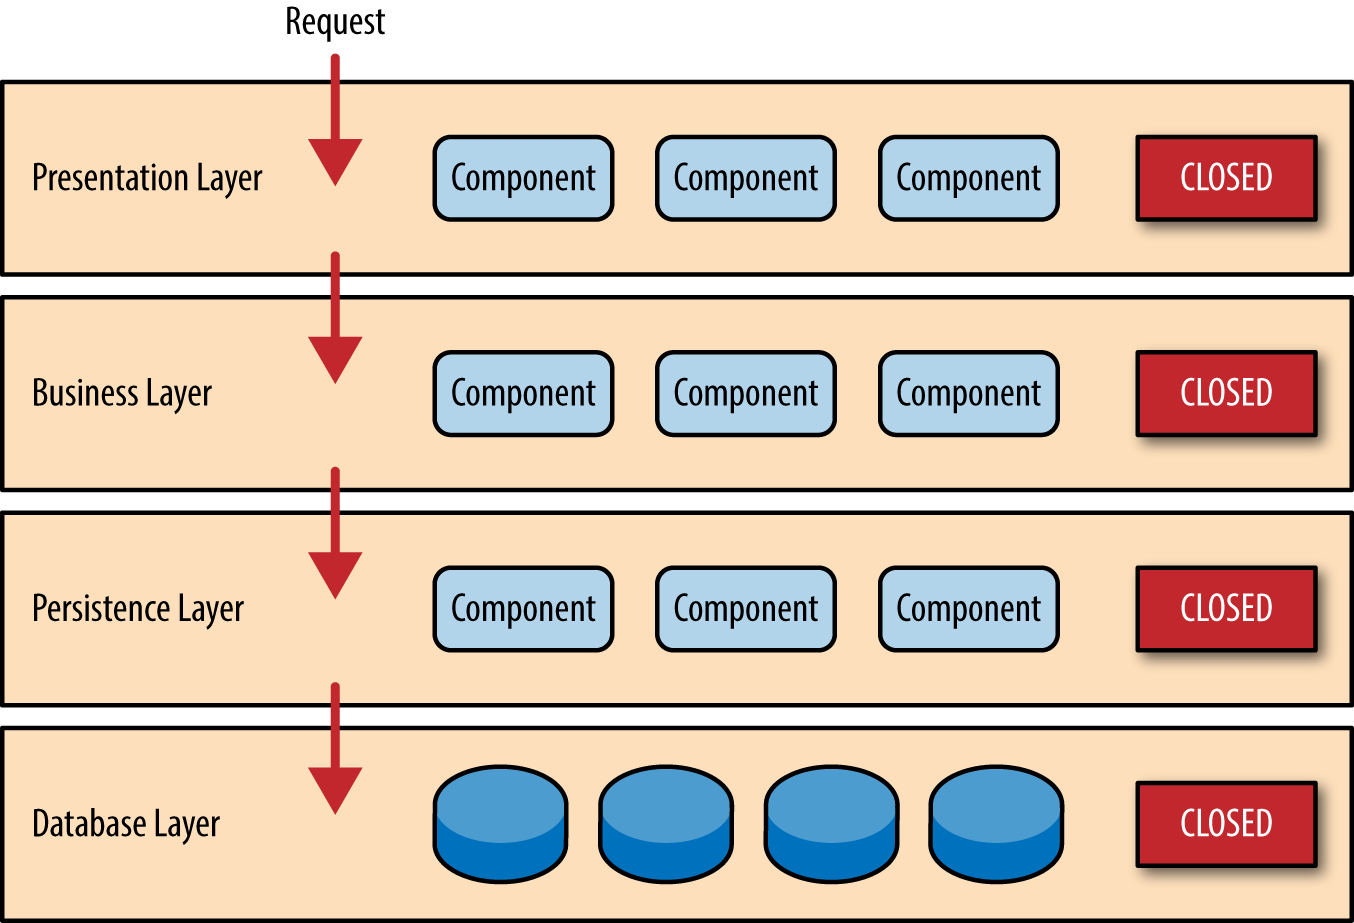
\includegraphics[height=6cm]{layered-architecture}
\end{figure}
\leavevmode\newline
Solitamente ogni livello comunica solo con il livello sottostante. Il connettore tra ogni livello può 
essere una chiamata di funzione, una richiesta di query, un oggetto dati o qualsiasi connettore che
trasmetta richieste o informazioni.
\\
La denominazione dei livelli è abbastanza flessibile ma di solito sono sempre presenti almeno: un livello di presentazione, un livello
di business e un livello fisico.
\\\\\\
\textbf{Livello di presentazione}
\\\\
Il livello di presentazione contiene tutte le classi responsabili di presentare la visualizzazione delle
delle informazioni all'utente finale. Idealmente questo è il solo livello con cui l'utente finale 
interagisce direttamente.
\\\\\\
\textbf{Livello di business}
\\\\
Il livello di business contiene tutta la logica che è richiesta dall'applicazione per poter soddisfare i 
suoi requisiti funzionali. Solitamente questo livello si occupa dell'aggregazione dei dati, della computazione
e della richiesta dei dati. Quindi qui è dove viene implementata la logica principale dell'applicazione.
\\\\\\
\textbf{Livello fisico}
\\\\
Qui è dove sono salvati tutti i dati recuperabili dell'applicazione. Solitamente questo livello è chiamato
anche livello di persistenza. Questo livello si occupa di interagire con il sistema in cui i dati 
sono mantenuti in maniera persistente, come ad esempio un database.

\subsection{Motivazioni della scelta}
Le motivazione che hanno portato a scegliere questo stile architetturale sono le seguenti:
\begin{itemize}
    \item Dato che la separazione delle responsabilità è la proprietà principale di quest'architettura,
        ogni livello di software ha la sua specifica funzione. Questo rende facile il dover aggiornare 
        singoli livelli e permette al team di sviluppo di separare bene i carichi di lavoro tra i vari 
        membri, che possono lavorare in maniera contemporanea su livelli diversi.
    \item Per la proponente è importante avere una suite di test automatici per testare i vari componenti
        dell'applicazione. La layered architecture separando bene le responsabilità tra i livelli, 
        permette di suddividere l'applicazione in componenti ben separati e quindi più facili da testare.
        Essendo ogni livello isolato dagli altri, è possibile creare casi di test di dimensione ridotta, 
        in quanto le componenti di cui fare il mock sono poche.
    \item L'isolamento tra i vari livelli permette di modificare un livello senza che la modifica intacchi
        gli altri livelli.
    \item Nel caso l'applicazione diventi molto grande è possibile, senza troppo sforzo, avviare un processo
        di migrazione ad un'architettura a microservizi. La layered architecture lavora bene (lato monolite) anche
        in un sistema con un'architettura ibrida monolite/microservizi. Questo tipo di architettura
        ibrida solitamente si forma nel processo di migrazione di un sistema monolitico in un sistema a microservizi.
        \\
        Di conseguenza, in ottica di una futura migrazione in un sistema a microservizi (molto probabile che avvenga), è
        bene scegliere un monolite che lavori bene in un'architettura ibrida e quindi che sia facile da migrare
        in un sistema a microservizi.
        \\
        Infatti grazie alla separazione delle responsabilità della layered architecture, è facile andare
        a trasformare i componenti del monolite in microservizi.
\end{itemize}

\section{Struttura software}
E' stato scelto NestJS come framework di sviluppo del progetto dato che utilizza la layered architecture,
tramite il pattern controller-service-repository. Vediamo questo design pattern:
\begin{figure}[!h]
    \centering
    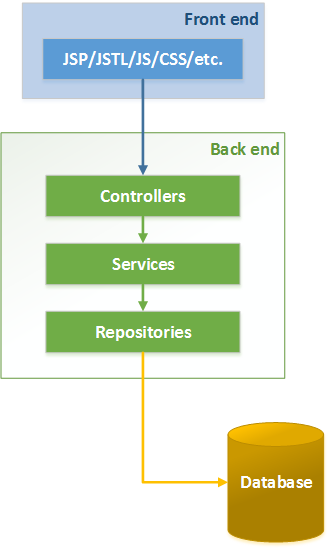
\includegraphics[height=6cm]{controller-service-repository-pattern}
\end{figure}
\leavevmode\newline
Il controller-service-repository pattern suddivide i componenti dell'applicazione su tre livelli fondamentali:
il controller, il service e il repository.
\\
Il controller è il livello più alto, mentre il repository quello più basso, in mezzo ai due c'è il service.
\\
Il controller è il livello responsabile per gestire le richieste in arrivo e ritornare le risposte all'utente finale.
Esiste un meccanismo di routing che gestisce a quale controller inviare le richieste.
\\
Il service è il livello responsabile della business logic.
\\
Il repository è il livello che viene anche chiamato livello di persistenza nella layered architecture e quindi interagisce
con il sistema di persistenza dati, come il database.
\\\\
Analizziamo in dettaglio le componenti che vanno a formare struttura del software:

\subsection{IoC container}
L'Inversion of Control container è un componente fondamentale di NestJS che permette l'applicabilità
del pattern Dependency Injection all'interno di NestJS.
\\
L'IoC container contiene un'istanza di tipo singleton per ogni classe dichiarata come controller o provider.
\\\\
Il funzionamento dell'IoC container è il seguente:
\\\\
quando viene avviata un'applicazione NestJS, il sistema runtime ricerca tutti controller e provider che 
sono stati dichiarati all'interno di moduli importati dal modulo root. Per ognuna di queste classi crea un'istanza
usando il pattern singleton e la inserisce nell'IoC container. 
\\
Se però la classe da istanziare dichiara una dipendenza con un altro controller o provider nel proprio 
costruttore, il sistema runtime applica in maniera automatica il pattern Dependency Injection; ovvero
va a cercare un'istanza della dipendenza dichiarata nel costruttore della classe, nell'IoC container, se
presente la inietta nella classe e crea l'istanza della nuova classe da inserire nell'IoC container. 
\\
Altrimenti va a creare prima
l'istanza della classe che deve essere iniettata, prima della classe che dichiara la dipendenza (se possibile, in quanto la
classe da iniettare potrebbe a sua volta richiedere una dipendenza e in tal caso si segue la successione di 
dipendenze fino a che non si trova una classe che possa essere istanziata) e la inietta nella classe che dichiara
la dipendenza, poi crea un'istanza della classe che ha dichiarato la dipendenza e la inserisce nell'IoC container.

\subsection{Controller e provider}
I due componenti fondamentali di NestJS sono i controller e i provider. 
Per dichiarare una classe come controller, bisogna applicare il decorator @Controller, sopra la 
definizione della classe, mentre per dichiarare una classe come provider bisogna applicare il decorator
@Injectable sopra la definizione della classe.
\\
\begin{lstlisting}
@Injectable()
export class MaintainersRegistryService {
    constructor(private readonly maintainersRegistryRepository: 
        MaintainersRegistryRepository){}

    getAllMaintainers(){
        return this.maintainersRegistryRepository.find();
    }

    async getMaintainerById(id: string){
        const maintainer = 
            await this.maintainersRegistryRepository.findOne({
                where: {
                    id: id
                }
            });

        if(isEmpty(maintainer))
            throw new NotFoundError('maintainer id not found');

        return maintainer;
    }

    async createMaintainer(maintainer: MaintainerRegistry){
        const insertResponse = 
            await this.maintainersRegistryRepository.insert(maintainer);

        if(isEmpty(insertResponse.identifiers))
            throw new InsertError('problem to insert record');

        const maintainerInsertedId = insertResponse.identifiers[0].id;

        return this.getMaintainerById(maintainerInsertedId);
    }

    async editMaintainerById(id: string, maintainerRegistry: MaintainerRegistry){
        try{
            await this.getMaintainerById(id);    
        }catch(error){
            throw(error);
        }
        
        const updateResponse = 
            await this.maintainersRegistryRepository.update(id, maintainerRegistry);

        const numberRowAffected = updateResponse.affected;

        if(numberRowAffected !== 1)
            throw new UpdateError('problem to update record');

        return this.getMaintainerById(id);
    }

    async deleteMaintainerById(id: string){
        try{
            await this.getMaintainerById(id);    
        }catch(error){
            throw(error);
        }

        const deleteResponse = 
            await this.maintainersRegistryRepository.delete(id);

        const numberRowAffected = deleteResponse.affected;

        if(numberRowAffected !== 1)
            throw new DeleteError('problem to delete record');
    }
}
\end{lstlisting}
\leavevmode\newline
\\
I controller sono i componenti dedicati a gestire le richieste in ingresso e a fornire le risposte all'utente
finale. NestJS considera come provider tutte le classi istanziabili e marcate con il decorator 
@Injectable che non sono controller; quindi sia classi di tipo service, che repository devono essere marcate
con il decorator @Injectable. 
\\
\begin{lstlisting}
@Controller('maintainers')
export class MaintainersRegistryController {
    constructor(private readonly maintainersRegistryService: 
        MaintainersRegistryService){}

    @Get()
    getAllMaintainers(){
        return this.maintainersRegistryService
            .getAllMaintainers();
    }

    @Get(':id')
    getMaintainerById(@Param('id') id: string){
        return this.maintainersRegistryService
            .getMaintainerById(id);
    }

    @Post()
    async createMaintainer(@Body() maintainer: MaintainerRegistry){
        return await this.maintainersRegistryService
            .createMaintainer(maintainer);
    }

    @Put(':id')
    editMaintainerById(
        @Param('id') id: string,
        @Body() maintainerRegistry: MaintainerRegistry,
    ){
        return this.maintainersRegistryService
            .editMaintainerById(id, maintainerRegistry);
    }

    @Delete(':id')
    @HttpCode(204)
    deleteMaintainerById(@Param('id') id: string){
        return this.maintainersRegistryService
            .deleteMaintainerById(id);
    }
}
\end{lstlisting}
\leavevmode\newline
\\
E' possibile marcare con il decorator @Injectable
anche classi non service o repository per fare in modo che NestJS, in maniera automatica, istanzi, inietti le dipendenze 
dichiarate nel costruttore e le inserisca nell'IoC container.
\\\\
I controller dell'applicazione individuati sono i seguenti:
\begin{itemize}
    \item MaintainersRegistryController: gestisce le richieste/risposte relative al dominio dei manutentori.
    \item ParkingAreasController: gestisce le richieste/risposte relative al dominio dei parcheggi.
    \item ParkingSensorsController: gestisce le richieste/risposte relative al dominio delle misurazioni
    dei sensori di parcheggio.
    \item ParkingSensorsSensorsController: gestisce le richieste/risposte relative al dominio delle misurazioni
    dei sensori di parcheggio di un sensore.
    \item ParkingSpotsController: gestisce le richieste/risposte relative al dominio delle piazzole.
    \item ParkingSpotsParkingAreasController: gestisce le richieste/risposte relative al dominio delle piazzole
    di un parcheggio.
    \item ParkingSpotsSensorsController: gestisce le richieste/risposte relative al dominio delle piazzole
    di un sensore.
    \item SensorsController: gestisce le richieste/risposte relative al dominio dei sensori.
    \item SensorsParkingSpotsController: gestisce le richieste/risposte relative al dominio dei sensori di una
    piazzola.
    \item SensorsMaintenanceSensorsController: gestisce le richieste/risposte relative al dominio della manutenzione dei
    sensori di un sensore.
\end{itemize}
% //TODO: inserire i service individuati
\subsection{Repository}
I repository sono i componenti dedicati alla gestione della persistenza dei dati. Hanno quindi il compito di
comunicare con la componente di archiviazione dati come un database. Nel progetto è stato utilizzato un database
relazionale di tipo postgreSQL.
\\\\
NestJS è indipendente dal tipo di database scelto (relazionale o non relazionale). Infatti NestJS si interfaccia
al database tramite uno strumento che si chiama TypeORM. TypeORM implementa una tecnica di programmazione chiamata 
ORM, che converte i dati tra diversi tipi di sistemi usando linguaggi di programmazione OOP.
\\\\
Uno strumento ORM incapsula il codice necessario per manipolare i dati, senza aver bisogno di scrivere manualmente
le query al database ma si interagisce direttamente con un oggetto nello stesso linguaggio che si sta usando. 
\\
In questo modo il database viene astratto e si diventa indipendenti dal tipo di database utilizzato, in quanto è compito dell'ORM
tradurre la richiesta fatta, in linguaggio di programmazione ad alto livello, nella query al database. 
\\\\
Uno strumento come TypeORM offre quindi una grande flessibilità, in quanto è possibile decidere di passare da un database
relazionale a un database non relazionale in qualsiasi momento, senza dover effettuare modifiche al livello di persistenza.
\\\\
Senza un'ORM la migrazione da un database relazionale a un database non relazionale implica la riscrittura di tutte le query.
\\\\
Il repository viene fornito e creato in maniera automatica da NestJS. Per fare in modo che ciò avvenga è però necessario
dichiarare, all'interno del modulo in cui si vuole che NestJS crei il repository e in particolare nell'array di imports, con 
il metodo forFeature della classe TypeOrmModule, la lista di entità di cui si vuole creare un repository.
\\\\
Il repository creato da NestJS include tutti i metodi necessari per le operazioni basilari CRUD (find(), save(), update(), 
delete() ecc..).
\\\\
Spesso però abbiamo bisogno di effettuare query al database più complesse rispetto a quelle a disposizione nel repository
creato da NestJS. Per fare ciò dobbiamo creare una nostra classe repository custom che estenda la classe Repository, che è una
classe Generic definita all'interno di NestJS e si aspetta come tipo del Generic il tipo dell'entità di cui vogliamo 
creare il repository.
\\\\
Se creiamo un repository custom non è più necessario usare il metodo forFeature nella classe modulo, ma va importato il repository custom
come provider.
\\ 

\begin{lstlisting}
@Injectable()
export class SensorsRepository extends Repository<Sensor>{
    constructor(private dataSource: DataSource){
        super(Sensor, dataSource.createEntityManager());
    }

    getSensorsWithoutSensorMaintenance(){
        return this.dataSource
        .createQueryBuilder()
        .select('sensor')
        .from(Sensor, 'sensor')
        .leftJoin('sensor.sensorMaintenance', 'sensorMaintenance')
        .where('sensorMaintenance.id IS NULL')
        .getMany();
    }
}
\end{lstlisting}
\leavevmode\newline
Nel repository custom, oltre che ai metodi ereditati dalla classe padre Repository, possiamo creare i nostri metodi personalizzati
che eseguono le nostre query custom. 
\\\\
Ci sono 2 modi per creare le query:
\begin{itemize}
    \item tramite notazione pura SQL;
    \item tramite i metodi del Query Builder;
\end{itemize}
\leavevmode\newline
E' fortemente consigliato l'utilizzo del Query Builder anziché usare la notazione SQL pura per 2 motivi:
\begin{enumerate}
    \item La concatenazione dei metodi del Query Builder rende molto più chiaro e pulito il codice, quindi più facile
        da manutenere.
    \item Nel caso di cambio di tipo di database (ad esempio passando da PostgreSQL a Oracle) le query continuano a funzionare, in 
        quanto grazie al Query Builder,
        TypeORM le converte adattandole alla sintassi del database che si stà utilizzando. Mentre non viene 
        effettuata alcun tipo di conversione per le query in notazione pura SQL.
\end{enumerate}
\leavevmode\newline
I repository custom dell'applicazione individuati sono i seguenti:
\begin{itemize}
    \item ParkingSensorsRepository: ha un metodo custom per aggiornare i timestamp delle misurazioni dei sensori di parcheggio 
        passate come parametro.
    \item SensorsRepository: ha un metodo custom per ottenere i sensori che non hanno almeno una manutenzione.
\end{itemize}
% rel: https://it.wikipedia.org/wiki/Object-relational_mapping

\subsection{Moduli}
Un modulo è una componente fondamentale di NestJS. Ogni applicazione ha almeno un modulo, chiamato modulo root. 
Avere solo un modulo non è un caso tipico per un'applicazione, solitamente ce ne sono molti.
I moduli sono utilizzati per organizzare i componenti di un'applicazione.
\\\\
All'interno di uno stesso modulo devono essere presenti componenti appartenenti allo stesso dominio. Ad esempio
il controller, il service e il repository dei sensori di parcheggio sono tre buoni candidati per essere racchiusi 
all'interno dello stesso modulo.
\\\\
Grazie ai moduli si riesce a mantenere il codice ben organizzato, separando le componenti per dominio di appartenenza
e stabilendo dei confini chiari tra i vari componenti. In questo modo NestJS ci aiuta a gestire la complessità e a 
sviluppare con principi SOLID, specialmente quando le dimensioni dell'applicazione crescono e/o quando il team cresce.
\\\\
In un modulo possiamo inserire solo componenti controller o provider. Per inserire un componente in un modulo, dobbiamo
specificare il nome del componente all'interno del decorator
@Module della classe modulo (i controller devono essere dichiarati nell'array controllers di all'interno di @Module,
mentre i provider devono essere dichiarati nell'array providers all'interno di @Module). 
\\\\
Se un controller o un provider non è dichiarato in un modulo che viene incluso dal modulo
root, NestJS non istanzierà la classe del componente e non verrà inserito nell'IoC container.
\\\\
Un concetto fondamentale dei moduli è che le componenti (controller, service, repository, classi varie..) dichiarate 
come appartenenti ad un modulo hanno uno scope locale al modulo, quindi sono visibili solo tra di loro e non vedono
i componenti appartenenti ad altri moduli.
\\
E' un caso comune però che un componente di un modulo abbia bisogno di un componente appartenente ad un altro modulo
e quindi lo dichiara come dipendenza. Facendo una cosa del genere NestJS genera un errore in fase di compilazione, poiché come 
spiegato sopra, un componente di un modulo A, non può vedere un componente di un modulo B.
\\\\
Per risolvere questo problema NestJS permette di definire nel decorator @Module della classe modulo, i componenti che
quel modulo vuole esportare e quindi che abbiano visibilità pubblica (i componenti da esportare devono essere dichiarati 
nell'array exports all'interno di @Module). 
\\
In questo caso se un componente di un modulo B dichiara una 
dipendenza da un componente esportato da un modulo A, nel decorator @Module, della classe modulo B, deve essere dichiarato il
modulo del componente che si vuole importare (i moduli da importare devono essere dichiarati nell'array imports all'interno di @Module).
\\
% //TODO: sistemare colori codice
\begin{lstlisting}
@Module({
    imports: [ 
        SensorsModule,
    ],
    controllers: [
        ParkingSpotsController, 
        ParkingSpotsParkingAreasController,
        ParkingSpotsSensorsController,
    ],
    providers: [
        ParkingSpotsService,
        ParkingSpotsRepository,
    ],
    exports: [
        ParkingSpotsService,
    ],
})
export class ParkingSpotsModule {}
\end{lstlisting}
\leavevmode\newline
I moduli dell'applicazione individuati sono i seguenti:
\begin{itemize}
    \item AutomapperCustomModule: contiene i componenti per effettuare il mappaggio da DTO a entità.
    \item DtoValidatorModule: contiene i componenti per validare i campi di un DTO.
    \item MaintainersRegistryModule: contiene i componenti appartenenti al dominio dei manutentori.
    \item ParkingAreasModule: contiene i componenti appartenenti al dominio dei parcheggi.
    \item ParkingSensorsModule: contiene i componenti appartenenti al dominio delle misurazioni dei sensori di parcheggio.
    \item ParkingSpotsModule: contiene i componenti appartenenti al dominio delle piazzole.
    \item SensorsModule: contiene i componenti appartenenti al dominio dei sensori.
    \item SensorsMaintenanceModule: contiene i componenti appartenenti al dominio della manutenzione dei sensori.
    \item SensorsScrapingModule: contiene i componenti appartenenti al dominio del polling dei sensori.
\end{itemize}

\subsection{DTO}
E' stata usata una classe di tipo DTO chiama SensorsScrapingDto. Questa classe viene utilizzata per rappresentare
il contenuto del file XML online contente lo stato dei sensori. Da questo oggetto vengono estratte le informazioni
utili per rappresentare le entità di tipo sensore e misurazioni sensore con cui si va ad aggiornare il database.
\\\\
Prima di effettuare la conversione da DTO a entità, i campi del DTO vengono validati, lanciando un'eccezione nel caso 
la validazione fallisca.
\\
\begin{lstlisting}
export class SensorScrapingDto{
    
    id: string;

    name: string;

    address: string;

    lat: string;

    lng: string;

    state: boolean;

    battery: string;

    active: boolean;

    constructor(){
        this.id = '0';
        this.name = '';
        this.address = '';
        this.lat = '0';
        this.lng = '0';
        this.state = false;
        this.battery = '';
        this.active = false;
    }
}
\end{lstlisting}

\subsection{Eccezioni}
NestJS ha un livello built-in che è responsabile di processare tutte le eccezioni non catturate durante 
l'esecuzione di un'applicazione.
\\\\
Quando un'eccezione non viene catturata dal codice dell'applicazione, viene catturata da questo livello,
che in maniera automatica invia una risposta user-friendly http al client, evitando di far interrompere 
l'esecuzione del programma. Questa componente si chiama exception filter.
\\\\
La risposta inviata al client dall'exception filter è user-friendly e contiene un messaggio appropriato, solo se l'eccezione è di tipo HttpException o 
una sua sottoclasse. 
Altrimenti viene inviata una risposta al client con un messaggio "internal server error" e status code 500.
\\\\
Possono capitare eccezioni anche durante l'esecuzione di query tramite TypeORM. Essendo TypeORM una libreria
esterna, nessuna eccezione da lei lanciata viene catturata dal livello descritto sopra di NestJS.
\\\\
Per evitare di interrompere l'esecuzione del programma al lancio di eccezioni non catturabili dall'exception filter di NestJS,
 si è deciso di 
sovrascrivere l'exception filter globale fornito da NestJS con uno custom e di creare un set di eccezioni
custom che vengono lanciate per problemi collegati al servizio di persistenza.
\\\\
Questo exception filter è stato chiamato TypeOrmExceptionFilter e implementa l'interfaccia ExceptionFilter di
NestJS. 
\\
TypeOrmExceptionFilter simula il comportamento dell'exception filter di NestJS catturando qualsiasi
tipo di eccezione, rispondendo con "internal server error" e status code 500 in caso l'eccezione non sia riconosciuta.
Inoltre funziona anche se si verificano eccezioni da librerie esterne; garantendo un buon livello di resilienza
del programma. 
\\\\
Se l'eccezione lanciata è quella custom, definita per i problemi del servizio di persistenza, lo status code e il messaggio 
vengono inviati in maniera
appropriata all'utente finale.
\\\\
Eccezioni di TypeORM di tipo QueryFailedError, vengono analizzate in base al loro codice di errore; 
lo status code e il messaggio anche in questo caso vengono inviati in maniera appropriata all'utente finale.
Un esempio di eccezione di tipo QueryFailedError con codice errore 23505, indica un confitto nel database, quindi
viene inviata una risposta al client con status code 409 e messaggio "database error on unique constraint".
\\\\
Avere un exception filter permette di spostare la responsabilità della gestione delle eccezioni in un livello
apposito. In questo modo si facilita la manutenzione e si assicura coerenza nella gestione delle eccezioni.
\\\\
Senza un exception filter dovrebbero essere i controller a gestire le eccezioni e modificare la loro risposta
in base al tipo di eccezione ricevuta dal service (che ha usufruito del metodo del repository che ha lanciato
l'eccezione).
\\\\
In questo modo però si creano controller di grandi dimensioni rendendo il codice meno pulito e più difficile
da manutenere. Inoltre questo approccio non garantisce che tutti i controller gestiscano la stessa eccezione
allo stesso modo. 
\\
Ad esempio sviluppatori diversi potrebbero gestire in maniera diversa la stessa eccezione (ad esempio rispondendo
all'utente finale con un messaggio di errore diverso,
più messaggi di errore, inserendo un numero e tipo di parametri di risposta diversi ecc..)
generando confusione per l'utente finale.
\\\\
Le eccezioni custom per TypeORM individuate sono le seguenti:
\begin{itemize}
    \item NotFoundError: gestisce errori dovuti alla richiesta di dati inesistenti.
    \item InsertError: gestisce errori dovuti all'inserimento di dati.
    \item UpdateError: gestisce errori dovuti all'aggiornamento di dati.
    \item DeleteError: gestisce errori dovuti alla cancellazione di dati.
\end{itemize}
\leavevmode\newline

\subsection{Scheduler}
Si è deciso di implementare il polling dei dati del sensore dal file XML online
tramite la libreria @nestjs/schedule che integra il package cron di Node.js.
\\\\
Questa libreria mette a disposizione uno strumento per poter eseguire il metodo
di una classe ad intervalli di tempo regolari.
\\\\
Per fare ciò bisogna importare nel modulo root, il modulo della libreria schedule in questo modo:
\begin{lstlisting}
@Module({
  imports: [
    ScheduleModule.forRoot()
  ],
})
export class AppModule {}
\end{lstlisting}
\leavevmode\newline
Successivamente abbiamo a disposizione un decorator @Cron, da indicare sopra al metodo che vogliamo venga 
schedulato. 
\\\\
Come parametro del @Cron dobbiamo inserire la stringa, rispettando il cron pattern, che indica
l'intervallo di tempo con cui vogliamo che NestJS esegua il metodo.
\\\\
Nel nostro caso vogliamo eseguirlo ogni due minuti quindi gli passiamo la stringa "*/2 * * * *".

\subsection{Logging}
Il logging in un'applicazione è un processo fondamentale che serve a salvare gli eventi che accadono durante
la sua esecuzione.
\\\\
Con queste informazioni in mano, gli sviluppatori possono accorgersi di potenziali attacchi o analizzare gli
errori prima che questi interrompano i flussi di lavoro aziendali.
\\\\
Il logging viene effettuato salvando su un file (solitamente con estensione .log) le informazioni rilevanti
accadute in un particolare evento di cui si è deciso di effettuare il logging, come la richiesta da parte
dell'utente finale di un servizio dell'applicazione.
\\\\
Solitamente questi file di log diventano molto grandi, quindi possono aver bisogno di un server dedicato per 
memorizzarli.
\\\\
Per questo progetto è stato deciso di fare il logging di tutte le richieste alle REST API da parte dell'utente
finale e tutte le volte che viene eseguito il servizio di polling schedulato.
\\
In particolare per le richieste alle REST API dell'utente finale si vuole effettuare il logging delle seguenti 
informazioni:
\begin{itemize}
    \item metodo della richiesta (GET, POST, PUT, DELETE);
    \item endpoint richiesto;
    \item corpo della richiesta;
    \item user agent dell'utente finale;
    \item ip dell'utente finale;
    \item status code di risposta;
    \item lunghezza del messaggio di risposta;
    \item timestamp della richiesta;
\end{itemize}
\leavevmode\newline
Per il servizio di polling si vogliono salvare le seguenti informazioni:
\begin{itemize}
    \item timestamp del momento di avvio del polling;
    \item timestamp del momento di fine del polling;
\end{itemize}
\leavevmode\newline

NestJS integra al suo interno una semplice classe logger che è possibile usare per effettuare il logging 
dell'applicazione. 
\\\\
Questa classe permette solo di effettuare operazioni basilari e come descritto nella 
guida ufficiale, per effettuare operazioni più complesse come il salvataggio delle informazioni di 
logging su file è bene appoggiarsi ad una libreria esterna che si integra molto bene con NestJS, chiamata
Winston.
\\\\
Con Winston è possibile definire l'output dei nostri log (nel nostro caso un file .log in una directory logs nel
progetto) e la formattazione nel testo (nel nostro caso abbiamo usato una funzionalità di Winston che permette
di usare la stessa formattazione dei log di NestJS).
\\\\
Esistono vari livelli di informazioni di cui si può effettuare il logging tramite winston. Il livello del log 
indica la sua importanza:
\begin{itemize}
    \item error: log critico, qualcosa nell'applicazione non ha funzionato correttamente e
        alcune funzionalità dell'applicazione potrebbero non funzionare correttamente;
    \item warn: log di avviso, qualcosa di inaspettato è successo nell'applicazione;
    \item info: log di informazione, è successo un evento all'interno dell'applicazione;
\end{itemize}
\leavevmode\newline
Esistono poi altri livelli di log che non sono stati però usti nel progetto, quindi si è deciso di non elencarli.
\\\\
Winston permette di scegliere a che livello registrare i log, per questo progetto è stato effettuato il logging
a livello error e info.
\\\\
Le richieste dell'utente finale e il servizio di polling sono stati loggati come livello info.
\\\\
E' stato implementato un middleware LoggerMiddleware per intercettare tutte le richieste dell'utente finale, prima che 
vengano passate ai controller e salvarne i log.
\\\\
Per avere anche lo status code della risposta inviata all'utente finale dal controller, il LoggerMiddleware, imposta un 
listener sull'evento close del'oggetto response. In questo modo il log viene scritto solo quando il controller ha terminato di
gestire la richiesta e abbiamo tutti i dati a disposizione per poterla loggare.
% ref: https://www.loggly.com/use-cases/application-logging-best-practices/

\begin{lstlisting}
@Injectable()
export class LoggerMiddleware implements NestMiddleware {
  constructor(
    @Inject(WINSTON_MODULE_PROVIDER)
      private readonly logger: Logger
  ){}

  use(request: Request, response: Response, next: NextFunction): void {
    const { ip, method, originalUrl: url } = request;
    const userAgent = request.get('user-agent') || '';
    const body = JSON.stringify(request.body);

    response.on('close', () => {
      const { statusCode } = response;
      const contentLength = response.get('content-length');

      this.logger.info(
        `${method} ${url} ${body} ${statusCode} ${contentLength} - ${userAgent} ${ip}`
      );
    });

    next();
  }
}
\end{lstlisting}

\section{Servizio di polling}
Sono state proposte due varianti in cui sviluppare il servizio di polling. Queste due varianti riguardano il
modo in cui il servizio SensorsScrapingService, che si occupa di effettuare il polling dei dati dei sensori
da un file XML online, debba comunicare col servizio di persistenza.
\\\\
Le due varianti:
\begin{enumerate}
    \item Far comunicare il SensorsScrapingService col servizio di persistenza effettuando delle chiamate http 
        alle REST API di cui ha bisogno.
    \item Far comunicare il SensorsScrapingService direttamente col livello di servizio dei sensori e dei parcheggi.
\end{enumerate}
\leavevmode\newline

E' stato scelto il punto 2. Vediamo le motivazioni che hanno portato a effettuare questa scelta, analizzando pro e 
contro dei due rispettivi punti.
\\\\
Pro del punto 1
\begin{itemize}
    \item Far comunicare il SensorsScrapingService con un servizio il servizio di REST API, separa bene le responsabilità e 
        nel caso di migrazione a un applicazione basata su microservizi, il microservizi non deve cambiare il modo in cui interagisce
        con il servizio di persistenza, in quanto continua a chiamare le stesse REST API tramite il protocollo http.
\end{itemize}
\leavevmode\newline
Contro del punto 1
\begin{itemize}
    \item Come analizzato nella fase di analisi dei requisiti il SensorsScrapingService deve effettuare 720 chiamate http giornaliere
        per scaricare i dati dei sensori aggiornati. 
        \\
        Quindi come minimo deve effettuare 720 chiamate http giornaliere anche alle REST API, per verificare se ci sono sensori
        da aggiornare. 
        \\
        Nella pratica le chiamate http da fare sono di più poiché dopo aver verificato se ci sono sensori da aggiornare ed
        eventualmente aggiornarli, bisogna fare un'altra chiamata http alle REST API per verificare se ci sono anche misurazioni dei sensori
        da aggiornare ed eventualmente aggiornarle. 
        \\
        Questo poiché grazie al DTO i dati dei sensori e delle misurazioni dei sensori vengono suddivisi in due entità diverse e quindi 
        le chiamate http alle REST API da fare sono diverse, in quanto sensori e misurazioni dei sensori appartengono a domini diversi, quindi
        hanno diverse REST API dedicate.
        \\
        Il che porta il numero di chiamate http da effettuare al servizio di REST API, pari ad un minimo di 1440 giornaliere.
\end{itemize}

\leavevmode\newline
\section{REST API}
Tramite lo strumento Stoplight sono state progettate 22 REST API. Stoplight light è uno strumento molto buono realizzato
appositamente per progettare REST API.
\\\\
Essendo un servizio in cloud è accessibile a chiunque abbia necessità di avere la documentazione delle api da utilizzare.
\\\\
Stoplight permette di definire l'end point dell'api, il metodo della richiesta per accedere alla risorsa (GET, POST, PUT, DELETE ecc..),
eventuale corpo della richiesta da fornire, eventuale corpo della risposta, status code delle varie risposte e altre informazioni
utili a chi deve sviluppare le api o all'utente finale che deve effettuare le richieste.
\\\\
Definita un'api su Stoplight è possibile generare il mock della risposta, in questo modo gli sviluppatori front-end non hanno bisogno
di attendere che il back-end venga realizzato per sviluppare la parte di front-end.
\\\\
Le REST API, suddivise per dominio di appartenenza, sono le seguenti:
% //TODO: valutare se inserire anche i codici di errore
\\\\
Parcheggio
\\
\begin{table}
    \begin{tabular}{|p{3.2cm}|p{1.4cm}|p{1.3cm}|p{5.8cm}|} 
    \hline
    Endpoint & Metodo & Codice risposta & Descrizione \\ 
    \hline
    /parking-areas & GET & 200 & Restituisce tutti i parcheggi \\ 
    \hline
    /parking-areas & POST & 201 & Crea un parcheggio \\ 
    \hline
    /parking-areas/\{id\} & GET & 200 & Restituisce il parcheggio con l'id richiesto \\ 
    \hline
    /parking-areas/\{id\} & PUT & 200 & Modifica il parcheggio con l'id richiesto \\ 
    \hline
    /parking-areas/\{id\} & DELETE & 204 & Elimina il parcheggio con l'id richiesto \\ 
    \hline
    \end{tabular}
\end{table}
\leavevmode\newline
\\
Manutentore
\\
\begin{table}
    \begin{tabular}{|p{3.2cm}|p{1.4cm}|p{1.3cm}|p{5.8cm}|} 
    \hline
    Endpoint & Metodo & Codice risposta & Descrizione \\ 
    \hline
    /maintainers & GET & 200 & Restituisce tutti i manutentori \\ 
    \hline
    /maintainers & POST & 201 & Crea un manutentore \\ 
    \hline
    /maintainers/\{id\} & GET & 200 & Restituisce il manutentore con l'id richiesto \\ 
    \hline
    /maintainers/\{id\} & PUT & 200 & Modifica il manutentore con l'id richiesto \\ 
    \hline
    /maintainers/\{id\} & DELETE & 204 & Elimina il manutentore con l'id richiesto \\ 
    \hline
    \end{tabular}
\end{table}
\leavevmode\newline
\\
Sensore
\\
\begin{table}
    \begin{tabular}{|p{3.2cm}|p{1.4cm}|p{1.3cm}|p{5.8cm}|} 
    \hline
    Endpoint & Metodo & Codice risposta & Descrizione \\ 
    \hline
    /sensors & GET & 200 & Restituisce tutti i sensori \\ 
    \hline
    /sensors/\{id\} & GET & 200 & Restituisce il sensore con l'id richiesto \\ 
    \hline
    /sensors/sensors-maintenance & GET & 200 & Restituisce tutti i sensori con le loro informazioni sulla 
        manutenzione \\ 
    \hline
    /sensors/\{id\}/sensors-maintenance & GET & 200 & Restituisce il sensore con l'id richiesto con le sue 
        informazioni sulla manutenzione \\ 
    \hline
    /sensors/\{id\}/sensors-maintenance & PUT & 200 & Modifica le informazioni di manutenzione del sensore con
        l'id richiesto \\ 
    \hline
    /parking-spots/\{id\}/sensors & GET & 200 & Restituisce tutti i sensori della piazzola con l'id richiesto \\ 
    \hline
    \end{tabular}
\end{table}
\leavevmode\newline
\\
Piazzola
\\
\begin{table}
    \begin{tabular}{|p{3.2cm}|p{1.4cm}|p{1.3cm}|p{5.8cm}|} 
    \hline
    Endpoint & Metodo & Codice risposta & Descrizione \\ 
    \hline
    /parking-areas/\{id\}/parking-spots & GET & 200 & Restituisce tutte le piazzole del parcheggio con l'id 
    richiesto \\ 
    \hline
    /parking-areas/\{id\}/parking-spots & POST & 201 & Crea una piazzola associata al parcheggio con l'id 
    richiesto \\ 
    \hline
    /parking-spots/\{id\} & PUT & 200 & Modifica la piazzola con l'id richiesto \\ 
    \hline
    /parking-spots/\{id\} & DELETE & 200 & Elimina la piazzola con l'id richiesto \\ 
    \hline
    /sensors/\{id\}/parking-spots & GET & 200 & Restituisce tutte le piazzole del sensore con l'id 
    richiesto \\ 
    \hline
    \end{tabular}
\end{table}
\leavevmode\newline
\\
Misurazione sensore di parcheggio
\\
\begin{table}
    \begin{tabular}{|p{3.2cm}|p{1.4cm}|p{1.3cm}|p{5.8cm}|} 
    \hline
    Endpoint & Metodo & Codice risposta & Descrizione \\ 
    \hline
    /sensors/{id}/parking-sensors & GET & 200 & Restituisce tutte le misurazioni del sensore di parcheggio con l'id 
    richiesto (ogni sensore di parcheggio ha solo una misurazione: l'ultima effettuata) \\ 
    \hline
    \end{tabular}
\end{table}